\chapter{Atomic and Molecular Mass}

A proton and a neutron have about the same mass. An electron, on the
other hand, has much less mass: One neutron weighs about the same
amount as 2000 electrons. Thus, the mass of any object comes mostly
from the protons and neutrons in the nucleus of its atoms.\index{proton} \index{neutron}

We know how many protons an atom has by what element it is, but how do we know the number neutrons?

If you buy a balloon filled with helium, it will have two different
kinds of helium atoms: Most of the helium atoms will have 2 neutrons, but a
few will have only 1 neutron. We say that these are two different
\textit{isotopes} of helium. We call them helium-4 (or $^4He$) and
helium-3 (or $^3He$).  Isotopes are named for the sum of protons and
neutrons the atom has: helium-3 has 2 protons and 1 neutron.\index{isotopes}

Watch Khan Academy's \textbf{Atomic mass, number, and isotopes} at \url{https://www.khanacademy.org/science/chemistry/atomic-structure-and-properties/introduction-to-the-atom/v/atomic-number-mass-number-and-isotopes}

A hydrogen atom nearly always has just 1 proton and no neutrons. A
helium atom nearly always has 2 protons and 2 neutrons. So, if you
have a 100 hydrogen atoms and 100 helium atoms, the helium will have
about 4 times more mass than the hydrogen. We say ``Hydrogen is about
1 atomic mass unit(amu), and helium-4 is about 4 atomic mass
units.''\index{atomic mass unit}

What, precisely, is an atomic mass unit? It is defined as 1/12 of
the mass of a carbon-12 atom. Scientists have measured the mass of
helium-4, and it is about 4.0026 atomic mass units. (By the way, an
atomic mass unit is also called a \textit{dalton}.)

\pagebreak

Now you are ready to take a good look at the periodic table of
elements. Here is the version from Wikipedia:\index{periodic table of elements}

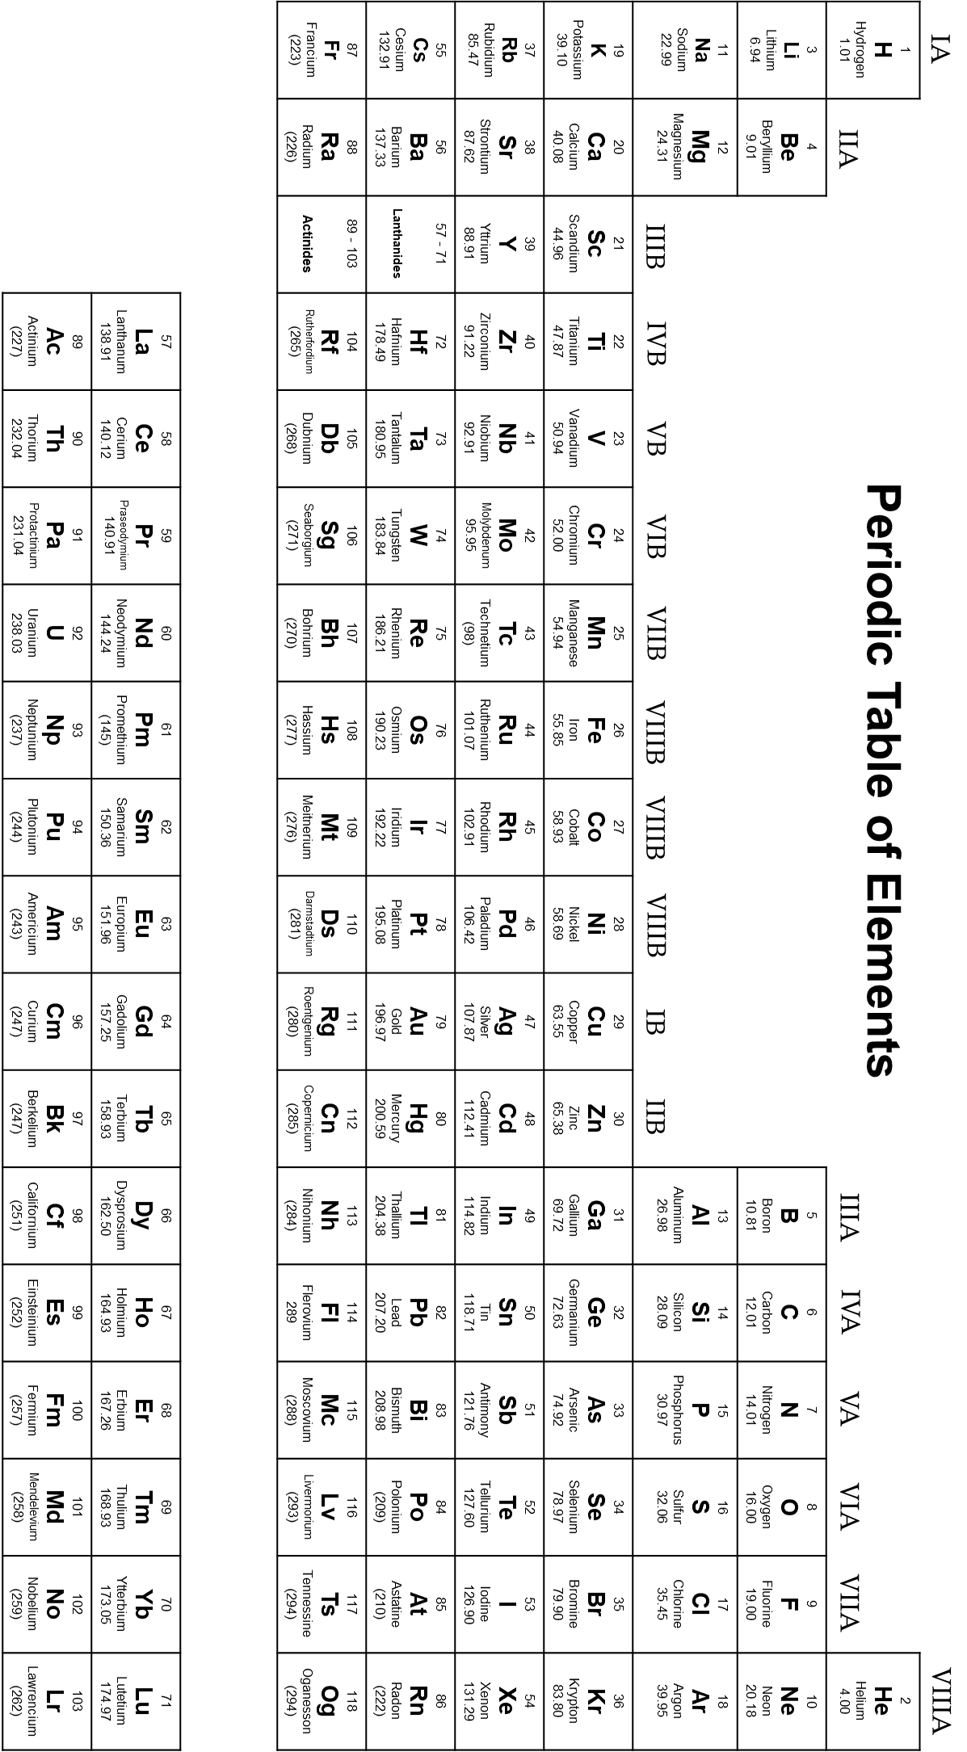
\includegraphics[width=0.75\textwidth]{periodic.png}

% ADD: Periodic Trends, Periods, Collums, Atomic Radius, Electronegativity,

\pagebreak
There is a square for each element. In the middle, you see the atomic
symbol and the name of the element. In the upper right corner is the
atomic number -- the number of protons in the atom.

In the upper left corner is the atomic mass in atomic mass units.\index{atomic mass}

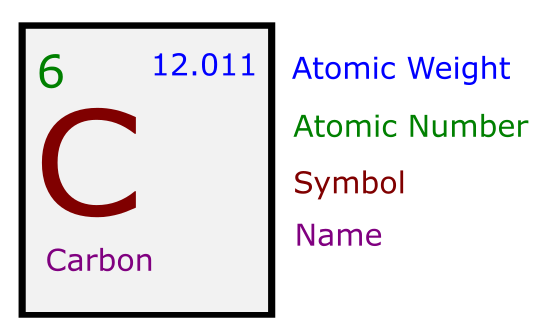
\includegraphics[width=0.8\textwidth]{Atomic_Carbon_Diagram.png}

Look at the atomic mass of boron. About 80\% of all boron atoms have
six neutrons. The other 20\% have only 5 neutrons. So most boron atoms
have a mass of about 11 atomic mass units, but some have a mass of
about 10 atomic mass units. The atomic mass of boron is equivalent to the average
mass of a boron atom: 10.811.
% ADD: Talk about mass spectroscopy
%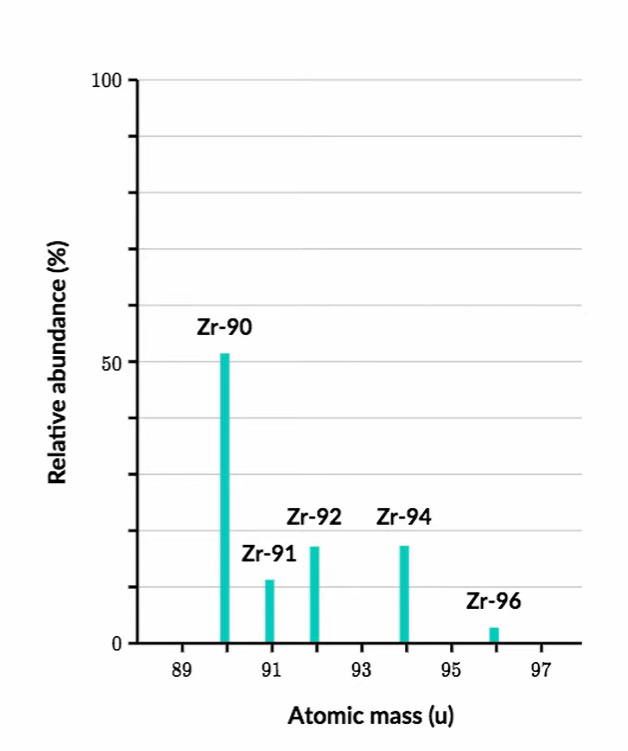
\includegraphics[width=0.75\textwidth]{KA_Mass_Spectroscopy_Zr.png}

\begin{Exercise}[title={Mass of a Water Molecule}, label=water_mass]
  
Using the periodic table, what is the average mass of one water molecule in atomic mass units?

\end{Exercise}
\begin{Answer}[ref=water_mass]

  The average hydrogen atom has a mass of 1.00794 atomic mass units.

  The average oxygen atom has a mass of 15.9994.

  $2 \times 1.00794 + 15.9994 = 18.01528$ atomic mass units.
   
\end{Answer}

\section{Molar Mass}

An atomic mass unit is a very, very, very small unit; we would much
rather work in grams.  It turns out that $6.02214076 \times 10^{23}$
atoms equal 1 mole( a standard measure for chemistry). Scientists use this number so much
that they gave it a name: \textit{the Avogadro constant} or
\textit{Avogadro's number}.\index{Avogadro's number}

Watch Khan Academy's discussion of the mole at \url{https://www.khanacademy.org/science/ap-chemistry-beta/x2eef969c74e0d802:atomic-structure-and-properties/x2eef969c74e0d802:moles-and-molar-mass/v/the-mole-and-avogadro-s-number}

If you have 12 doughnuts, that's a dozen doughnuts.  If you have
$6.02214076 \times 10^{23}$ doughnuts, you have a \textit{mole} of
doughnuts. (Note: it isn't practical to measure doughnuts this
way: A mole of doughnuts would be about the size of the earth. We use
moles for small things like molecules.)\index{mole}

Let's say you want to know how much a mole of $NaCl$ weighs. From the
periodic table, you see that $Na$ has an atomic mass of 22.98976
atomic mass units. And $Cl$ has 35.453 atomic mass units.  One atom of
$NaCl$ has a mass of $22.98976 + 35.453 = 58.44276$ atomic mass units.
Then a mole of $NaCl$ has a mass of $58.44276$ grams. Handy, right?
% ADD: Conversions should probably come before this

\begin{Exercise}[title={Burning Methane}, label=burning_methane]
  
Natural gas is mostly methane ($CH_4$). When one molecule of methane
burns, two oxygen molecules ($O_2$) are consumed. One molecule of
$H_2O$ and one molecule of $CO_2$ are produced.
% ADD: Need to explain mole to mole ratios first, Law of Divine Proportion
% ADD: Include Significant Figures

If I need 200 grams of water, how many grams of methane do I need
to burn?

(This is how the hero in ``The Martian'' made water for his garden.)

\end{Exercise}
\begin{Answer}[ref=burning_methane]

From the last exercise, you know that 1 mole of water weighs 18.01528
grams. So 200 grams of water is about 11.1 moles. So you need to burn
11.1 moles of methane.

What does one mole of methane weigh? Using the periodic table:
$12.0107 + 4 \times 1.00794 = 16.04246$ grams.

$16.0424 \times 11.10 = 178.1$ grams of methane.
   
\end{Answer}

\section{Heavy atoms aren't stable}

When you look at the periodic table, there are a surprisingly large
number of elements. You might be told to ``Drink milk so that you can
get the calcium you need.'' However, no one has told you ``You should
eat kale so that you get enough copernicium in your diet.''

Copernicium, with 112 protons and 173 neutrons, has only been observed
 in a lab. It is highly radioactive and unstable(meaning it decays): a copernicium
atom usually lives for less than a minute before decaying.
% ADD: Half Life

The largest stable element is lead, which has 82 protons and between
122 and 126 neutrons. Elements with lower atomic numbers than lead,
have at least one stable isotope. Elements with higher atomic numbers
than lead don't.

Bismuth, with an atomic number of 83, is \textit{almost} stable. In fact, most
bismuth atoms will live for billions of years before decaying.
